\documentclass{article}
\usepackage[T1]{fontenc}
\usepackage{scrextend}
\usepackage{glossaries}
\usepackage{minted}
\usepackage{graphicx}

\graphicspath{ {../img/} }

\makenoidxglossaries

\newglossaryentry{WLP}{name={WLP},description={Wektor Liczb Przeszukiwanych}}

\newglossaryentry{SE}{name={SE},description={Sito Erastotenesa}}

\newglossaryentry{PPLL}{name={PPLL},description={Pełny Przegląd Listy Liczb}}

\newglossaryentry{WLU}{name={WLU},description={Wektor Liczb Uporządkowanych}}

\newglossaryentry{TLP}{name={TLP},description={Tablica Liczb Pierwszch}}

\newglossaryentry{SPPLL}{name={SPPLL},description={Sekwencyjny Pełny Przegląd Listy Liczb}}

\newglossaryentry{RNPPLL}{name={RNPPLL},description={Równoległy Naiwny Pełny Przegląd Listy Liczb}}

\newglossaryentry{ROPPLL}{name={ROPPLL},description={Równoległy Naiwny Pełny Przegląd Listy Liczb}}

\newglossaryentry{SSE}{name={SSE},description={Sekwencyjne Sito Erastotenesa}}

\newglossaryentry{RNSED}{name={RNSED},description={Równoległe Naiwne Sito Erastotenesa w wersji Domenowej}}

\newglossaryentry{ROSED}{name={RNSED},description={Równoległe Optymalne Sito Erastotenesa w wersji Domenowej}}

\newglossaryentry{RNSEF}{name={RNSED}, description={Równoległe Naiwne Sito Erastotenesa w wersji Funkcyjnej}}

\newglossaryentry{ROSEF}{name={RNSED}, description={Równoległe Optymalne Sito Erastotenesa w wersji Funkcyjnej}}



\begin{document}
    \title{
        Sprawozdanie z Projektu Pierwszego \\
        \small{Laboratorium Przetwarzania Równoległego}
    }
    \author{
        \textbf{Piotr Tylczyński}\\
        \texttt{L7 / 141331} \\
        \texttt{Środa, 11:45} \\
        \texttt{piotr.tylczynski@student.put.poznan.pl}
        \and
        \textbf{Zuzanna Rękawek}\\
        \texttt{L7 / 141304} \\
        \texttt{Środa, 11:45} \\
        \texttt{zuzanna.rekawek@student.put.poznan.pl}
        \date{}
        }
    \begin{titlepage}
        \maketitle
        \centering{
            Oddane: 29.04.2021 \\
            Deadline: 29.04.2021 \\
        }
        \hfill \break
        \centering{Wersja 1}
            
            
    \end{titlepage}
    
    \tableofcontents
    \pagebreak
    
    \section{Motywacja}
        Celem niniejszego projketu jest stworzenie efektywnego programu wyszukującego liczby pierwsze w zadanym przedziale. W tym celu wykorzystamy porogramowanie równoległe. Pozwoli to na efektywniejsze wykorzystanie zasobów komputerowych jakimi dysponujemy. W wyniku otrzymamy program mogący wykorzystywać do 100\% mocy obliczeniowej procesora komputera, na którym zostanie uruchomiony. Pozwoli to nam na znaczącą redukcję czasu wykonania programu względem standardowej wersji sekwencyjnej programu.
        
        W rozwiązaniu wykorzystamy algorytm Sita Erastotenesa (\gls{SE}). Jest to algorytm pozwalający na osiągnięcie znaczącego przyspieszenia, po jego zrównolegleniu. Dodatkowo rozważymy wykorzystanie i zrównoleglanie algorytmu Pełnego Przeglądu List Liczb (\gls{PPLL}).
        
    \section{Uwagi Ogólne}
        Niestety po zakończeniu pisania tego sprawozdania zdaliśmy sobię sprawę z pewnego błędu jaki wkradł się podczas tworzenia i eksperymentowania z poszczególnymi algorytmami. Niestety pomyliliśmy ze sobą nazwy podejścia domenowego i funkcyjnego. Z tego powodu każde wystąpienie słowa \emph{domenowy} powinno zostać zastąpione słowem \emph{funkcyjny} i na odwrót.
        
    \section{Specyfikacja platformy uruchomieniowej}
        \begin{addmargin}{3em}
            \begin{description}
                \item[Procesor] Intel Core i5-9300H
                    \begin{description}
                        \item[Procesorów Fizycznych] 4
                        \item[Procesorów Logicznych]  8
                        \item[Pamięć Cache]  8 MB Intel® Smart Cache 
                    \end{description} 
                \item[System Operacyjny] Windows 10 Pro 20H2
                \item[IDE] Visual Studio 2019
                % TODO: check vtune version
                \item[Oprogramowanie Testujące] Intel®VTune\texttrademark Profiler
            \end{description}
        \end{addmargin}
        
    \section{Problemy i zjawiska występujące w programach równoległych}
        \subsection{Problemy Poprawnościowe}
            \subsubsection{Zjawisko wyścigu}
                Jest to zjawisko polegające na ubieganiu się o dostęp do pojedynczego zasobu przez wiele wątków. Jest to warunek konieczny wystąpienia w.w. zjawiska. Jeżeli nie zastosujemy, żadnego systemu zarządzania dostępem okaże się, że wynik wykonania programu nie będzie deterministyczny. Będzie to spowodowane przez używanie jednego zasobu przez wiele wątków. Będą one potencjalnie zapisywały do zasobu równocześnie. Spowoduje to, że wartość zapisana będzie w najlepszym przypadku wartością zapisaną przez ostatni wątek. W gorszym przypadku powstanie losowa kombinacja wartości zapisywanych przez poszczególne wątki. Kolejość informacji zapisanych w zasobie będzie zależała od czasu dostępu, stąd nazwa wyścig.
                
                Oczywiście występowanie zjawiska wyścigu nie jest porządana. Może ona doprowadzić do powstania złych wyników. W najgorszym przypadu będą one wypadkową, lub permutacją poprawnych wyników. 
                
                Rozwiązaniem problemu wyścigu jest wprowadzenie ograniczeń w dostępie do współdzielonego zasobu. W najprostszy sposób można to osiągnąć blokując zasób w czasie jego wykorzystywania przez wątek. Wtedy pozbędziemy się problemu wielodostępu i nigdy nie dopuścimy do spełnienia warunku koniecznego. Narzędziem, które może okazać się przydatne mogą być monitory, lub semafory. W naszym projekcie zastosujemy odpowiednie klauzule, które zapobiegną opisywanemu zjawisku. Będą to klauzule synchronizujące i dzielącę prace między wątkami, które zostały szczegółowo opisane poniżej, jaki i w opisach samych algorytmów.
        
        \subsection{Problemy Efektywnościowe}
            \subsubsection{Problem False Sharing}
                Polega na unieważnieniu potencjalnie nie współdzielonych danych w pmięci podręcznej procesora. Dzieje się tak, ponieważ leżą one na tej samej lini adresowej procesora. Z tego powodu jeżeli procesor wykonuje zapis do jednej z komórek pamięci to może się okazać, że narusza inną zmienną leżącą na tej samej lini pamięci. W takim wypadku, zmienna ta zostanie uznana za \emph{"brudną"} i będzie wymagała ponownego pobrania z pamięci.
                
                Zjawisko False Sharingu prowadzi do znaczengo spadku efektywności programu. W skrajnych przypadkach może okazać się, że program jest znacząco wolniejszy od swojej wersji sekwencyjnej. Jest to bezpośrednie następstwo wielokrotnego i niepotrzebnego unieważniania liń pamięci. Co sprawia, że wymagany jest dodatkowy narzut czasowy związnay z transferem danych pomiędzy poszczególnymi poziomami pamięci komputera.
                
                Rozwiązaniem problemu False Sharingu jest odpowiednia separacja przestrzenna danych. W przypadku tabel można to zapewnić przez umieszczenie wolnych miejsc pomiędzy danymi do zapisu. W ten sposób dane nie będą leżały na tej samej lini pamięci.
                
                W wyniku eksperymentu przeprowadzonego w ramach zadania pierwszego wyznaczyliśmy wielkość pojedyńczej lini pamięci na 64B
        
    \section{Zastosowane Algorytmy}
        \subsection{Opis teoretyczny}
            \subsubsection{Sito Erastotenesa}
                W swojej najprostszej formie \gls{SE} jest alogrytmem, który przyjmuje na swoje wejście wektor liczb naturalnych, uporządkowanych rosnąco z krokiem jeden - w dalszych częściach teog dokumentu nazywanych Wektorem Liczb Uporządkowanych - ()\gls{WLU}). Zastosowanie \gls{WLU} pozwala na dokonanie pewnej optymalizacji. Polega ona na sprawdzaniu tylko liczb znajdujących się przed połową takiego wektora. Optymalizacja taka jest możliwa, ponieważ \gls{WLU} jest rosnąco uporządkowany, więc wiemy, że wszystkie liczby złozone w drugiej połowie są, wielokrotnością, liczb znajdujących się w pierwszej połowie. Biorąc pod uwagę sposób działania algorytmu, który wykreśla z \gls{WLU} wszystkie wielokrotności liczb, mamy pewność, że po przejrzeniu wszystkich liczb z pierwszej połowy, wyeliminowaliśmy wszystkie pozostałe z drugiej połowy.
                
                Sam sposób działania \gls{SE} jest prosty. Dla każdej znalezionej liczby w \gls{WLU} wykreśl z \gls{WLU} wszystkie jej wielokrotności - w ten sposób pozbywamy się liczb złożonych. Następnie przejdź do kolejnej liczby w \gls{WLU} i powtórz poprzedni krok. Algorytm ten działa o ile przeglądamy liczby z zakresu 1 do N (N dowolna liczba całkowita). Jeżeli pierwszą liczbą w \gls{WLU} nie jest 1 to należy stworzyć sztuczny iterator, który będzie przechodził przez dodatkową tablicę zawierającą wszystkie liczby pierwsze (\gls{TLP}). Kolejną optymalizację jaką można dokonać jest ograniczenie wielkości tablicy liczb peirwszych. Maksymalna wymagana liczba pierwsza to pierwiastek kwadratowy z ostatniej liczby wchodzącej w skład \gls{WLU}. Tą własność można łatwo udowodnić, ponieważ największy dzielnik dowolnej liczby naturalnej nie może być większy niż pierwiastek kwadratowy z niej samej.
            
            \subsubsection{Przegląd Listy Liczb}
                Jest to jden z najprostszych algorytmów wyszukiwania liczb pierwszych. W swojej sekwencyjnej wersji polega na pełnym przejrzeniu \gls{WLU} i znalezieniu w nim liczb pierwszych. Jest to algorytm mniej skuteczny niż \gls{SE}, jednak szybszy w implementacji.
                
            \subsubsection{Określanie pierwszości liczyb}
                Działa na zasadzie iterowania się po wszystkich liczbach z zakresu 2 do wartości liczby. Jednocześnie sprawdzamy, czy któraś z liczb nie jest dzielnikiem sprawdzanej liczby. Jeżeli tak to wiemy, że dana liczba jesst liczbą złożoną. Po zakończeniu iterowania i nie znalezieniu dzielnika, możemy stwierdzić, że sprawdzana liczba jest pierwsza. Optymalizacja algorytmu polega na sprawdzaniu liczby tylko i wyłącznie nie większych niż pierwiastek kwadratowy z testowanej liczby. Uzasadnienie tego faktu można znaleźć w algorytmie \gls{SE}.
        \subsection{Realizacja praktyczna}
            \subsubsection{Wykorzystane klauzule OMP}
                \begin{description}
                    \item[\texttt{omp\_get\_max\_threads()}] podaje maksymalną dostępną w systemie liczbę procesorów logicznych
                    \item[\texttt{omp\_get\_wtime()}] zwraca czas pracy wszystkich wątków
                    \item[\texttt{\#pragma\ omp\ parallel}] rozpoczyna obszar wykonania Równoległego
                    \item[\texttt{\#pragma\ omp\ for}] pozwala na zrównoleglanie pętli dzieląc wykonywaną przez nią pracę pomiędzy dostępne wątli 
                    \item[\texttt{omp\_get\_thread\_num()}] zwraca numer aktualnie wykonywanego wątku
                    \item[\texttt{omp\_set\_num\_threads()}] ustawia maksymalną ilość wątków jakiej może używać program
                    \item[]   
                \end{description}
            \subsubsection{Sekwencyjne Określanie Pierwszości Liczb}
                Dokładne działanie algorytmu zostało zaprezentowane w części teoretycznej. Jedyną różnicą jest zastosowanie reszty z dzielenia jako metody określania dzielnika. Jeżeli wynikiem reszty z dzielenia jest zero to wiadomo, że $div$ jest jednym z dzielników liczby $p$, co oznacza, że liczba $p$ nie jest pierwsza.
                \begin{figure}[H]
                    \begin{minted}[linenos]{cpp}
bool isPrime(int p)
{
	int div = 2;
	double sqrtP = (int)sqrt(p) + 1;

	for (; div < sqrtP; ++div){ 
		if(p % div == 0) 
			return false;
	}

	return true;
}
                    \end{minted}
                    \caption{Sekwencyjne Określanie Pierwszości Liczb}
                \end{figure}
                
            \subsubsection{Sekwencyjny Pełny Przegląd Listy Liczb - \gls{SPPLL}}
            Tak jak opisano w części teoretycznej polega na pełnym przeglądzie wszystkich liczb z podanego zakresu. Aby zpoptymalizować wykonanie programu ustalamy wielkość wynikowego wektora na samym początku. Następnie w pętli sprawdzamy wszystkie liczby w zakresie od \emph{start} do \emph{end}. Samo sprawdzanie odbywa się w funkcji \emph{isPrime}, która została szczególowo opisana wcześniej.
                \begin{figure}[H]
                    \begin{minted}[linenos]{cpp}
std::vector<int> sequential::withoutSieve(int start, int end, bool printOutput){
    int size = end - start + 1;
    std::vector<int> result;
    double timeStart, timeStop;
                
    result.reserve(size);
    timeStart = omp_get_wtime();
    for (size_t i = start; i <= end; ++i){
        if (isPrime(i)) {
            result.push_back(i);
        }
    }
    timeStop = omp_get_wtime();
    if(printOutput) period(timeStart, timeStop, "sequential::withoutSieve");
                
    return result;
}
                    \end{minted}
                    \caption{Sekwecyjny Przegląd Listy Liczb}
                \end{figure}
                
            \subsubsection{Sekwencyjne Sito Erastotenesa - \gls{SSE}}
                Dokładne dziłanie tego algorytmu zostało także zaprezentowane w części teoretycznej. Algorytm rozpoczyna od wyznaczenia wszystkich liczb pierwszych, aż do pierwiastka górnej granicy przeszukiwania \emph{(wyjaśnienie w części teoretycznej)}. Następnie w pierwszej pętli $for$ usuwamy wszystkie wielokrotności kolejnych liczb pierwszych znajdujących się w tablicy $primes$. Jeżeli dana liczba została oznaczona jako $true$ to mamy pewność, że jest liczbą złożoną. Po sprawdzeniu ostatniej liczby z wektora $primes$, możemy przepisać wszystkie liczby, które nie zostały zakwalifikowane jako złożone.
                \begin{figure}
                    \begin{minted}[linenos]{cpp}
std::vector<int> sequential::withSieve(int start, int end, bool printOutput){
    int sqrtEnd = (int)sqrt(end);
    double timeStart, timeStop;
    timeStart = omp_get_wtime();
    std::vector<int> primes = sequential::withoutSieve(2, sqrtEnd, false);
    std::vector<bool> isPrime(end + 1, false);
    int primesSize = primes.size();
    for (auto& p: primes){
        int multiple = p * 2;
        while (multiple <= end) {
            isPrime[multiple] = true;
            multiple += p;
        }
    }
    int size = end - start + 1;
    std::vector<int> result;
    result.reserve(size);
    for (size_t i = start; i <= end; i++){
        if (!isPrime[i]) result.push_back(i);
    }
    timeStop = omp_get_wtime();
    if (printOutput) period(timeStart, timeStop, "sequential::withSieve");
        return result;
    return std::vector<int>();
}
                    \end{minted}
                    \caption{Sekwencyjne Sito Erastotenesa}
                \end{figure}
                
            \subsection{Równoległy Pelny Przegląd Listy Liczb}
                Zrównoleglenie Sekwencyjnego algorytmu Przeglądania Listy Liczb, opiera się na podziale \gls{WLU} pomiędzy wszystkie wątki. W takim wypadku każdy wątek będzie odpowiedzialny za przeszukiwanie swojej i tylko swojej części \gls{WLU}. Sercem algorytmu jest funkcja $isPrime$ wywoływana dla każdej liczby w celu sprawdzenia, czy jest pierwsza. Jeżeli taka jest to należy ją zapisać do wektora wyjściowego.
                \paragraph{Podejście Naiwne - \gls{RNPPLL}}
                    W wersji naiwnej algorytm zapisuje wyniki do jednowymiarowego wektora. Takie rozwiązanie nie jest poprawne. W skrajnych przypadkach może wystąpić zjawisko wyścigu. Okaże się, że istnieją momenty, w których wiele wątków stara się zapisać do wektora wynikowego efekty swojego przetwarzania. Spowoduje to, że wynikowy wektor może zostać łatwo uszkodzony. Dodatkowo program jest wrażliwy na wystąpienie zjawiska false sharingu. Nie spowoduje on niepoprawnego działania kodu, jednak znacząco wpłynie na prędkość przetwarzania. Stanie się tak, ponieważ elementy wekotra wyjściowego są ułożone w pamięci jeden obok drugiego, co łatwo prowadzi do uniważniania sąsiednich liń pamięci. 
                    \begin{minted}[linenos]{cpp}
std::vector<int> primes(int start, int end, bool printOutput){
    int size = end - start + 1;
    std::vector<int> result;
    double timeStart, timeStop;
    result.reserve(size);
    timeStart = omp_get_wtime();
#pragma omp parallel
    {
#pragma omp for
        for (int i = start; i <= end; i++){
            if (isPrime(i)) result.push_back(i);
        }
    }
    timeStop = omp_get_wtime();
    if (printOutput) period(timeStart, timeStop, "domain::primes");
    return result;
}
                    \end{minted}
                
                \paragraph{Podejście Optymalne - \gls{ROPPLL}}
                    Poprawa wersji naiwnej jest prosta. Wystarczy dodać strukturę pośrednią. W taki sposób, że wątki równolegle będą do niej zapisywać, a później w sposób sekwencyjny spłaszczymy ją do jednowymiarowego wektora. Wspomnianą strukturą może być dwuwymiarowy wektor. W takim wypadku każdy z procesów będzie zapisywał do swojego własnego wiersza, a na końcu w sposób sekwencyjny połączymy wszystkie wiersze w jedną tabelę.
                    
                    Zjawisko false sharingu nie zajdzie, ponieważ komórki pamięci będą znacząco od siebie oddzielone - conjmniej o jeden wiersz w wektorze. Zjawisko wyścigu także zostanie wyeliminowane. Żadne dwa wątki nie mogą zapisywać do tego samego wiersza, co oznacza, że mają swoje osobne przestrzenie robocze.
                \begin{figure}[H]
                    \begin{minted}[linenos]{cpp}
std::vector<int> primes(int start, int end, bool printOutput){
    int size = end - start + 1;
    std::vector<int> result;
    double timeStart, timeStop;
    int threadsCount = omp_get_max_threads();
    result.reserve(size);
    timeStart = omp_get_wtime();
    std::vector<std::vector<int>> privateResults(threadsCount, std::vector<int>());
    for (int i = 0; i < threadsCount; i++) privateResults[i].reserve(end - start + 1);
    #pragma omp parallel
    {
    #pragma omp for
        for (int i = start; i <= end; i++){
            if (isPrime(i))
                privateResults[omp_get_thread_num()].push_back(i);
        }
    }
    for (size_t i = 0; i < threadsCount; i++)
        result.insert(
            result.end(), privateResults[i].begin(), privateResults[i].end()
        );
    timeStop = omp_get_wtime();
    if (printOutput) period(timeStart, timeStop, "funcional::primes");
    return result;
}
                    \end{minted}
                    \caption{Optymalny Równoległy Przegląd Listy Liczb}
                \end{figure}
                
                
            \subsubsection{Równoległe Sito Erastotenesa - wersja domenowa}
                Zrównoleglenie \gls{SE} dla podejścia domenowego polega na przekazaniu całego \gls{WLU}, ale tylko części wektora liczb pierwszych. W taki sposób każdy wątek będzie odpowiedzialny za sprawdzenie, czy elementy \gls{WLU} są podzielne przez liczby pierwsze znane dla niego. Tak samo jak w sekwencyjnym \gls{SE} i tutaj można zastosować optymalizację w postaci ograniczenia największej liczby pierwszej do sprawdzenia do pierwiastka kwadratowego największej z liczb w \gls{WLU}.
                
                \paragraph{Podejście Naiwne - \gls{RNSED}}
                    W tej wersji naiwnej algorytmu rozpoczynamy od wygenerowania wszystkich potrzebnych liczb pierwszych. Następnie inicjalizujemy odpowiednio duży wektor przetrzymujący rozwiązanie. Następnie w pętli za pomocą odpowiedniej dyrektywy \emph{OMP} przydzielamy liczby pierwsze do wątków. Następnie każdy z wątków sprawdza całe \gls{WLU} w celu sprawdzenia, czy nie znajdują się w nim wielokrotości przydzielonych mu liczb pierwszych. Jeżeli takie występują to są oznaczane jako liczby pierwsze - wpis do wektora $isPrime$ wartości $true$ w odpowiednie miejsce. Na końcu powstały wektor $isPrime$ przetwarzamy na wektor wynikowy.
                    
                    Problemem wersji naiwnej jest niepoprawność generowanych wyników, oraz występujące zjawisko false sharingu - oba spowodowane używaniem wspólnej listy $isPrime$. Jego geneza jest dokładnie taka sama jak w przypadku naiwej wersji algorytmu \gls{PPLL}
                    \begin{figure}
                        \begin{minted}[linenos]{cpp}
std::vector<int> domain::basicSieve(int start, int end, bool printOutput){
    double timeStart, timeStop;
    int sqrtEnd = (int)sqrt(end);
    std::vector<int> primes =
         domain::primes(2, sqrtEnd, false);
    std::vector<bool> isPrime(end + 1, false);
    timeStart = omp_get_wtime();
#pragma omp parallel 
    {
#pragma omp for schedule(static)
        for (int i = 0; i < primes.size(); i++){
            int multiple = primes[i] * 2;
            while (multiple <= end) {
                isPrime[multiple] = true;
                multiple += primes[i];
            }
        }
    }
    int size = end - start + 1;
    std::vector<int> result;
    result.reserve(size);
    for (int i = start; i <= end; i++){
        if (!isPrime[i]) {
            result.push_back(i);
        }
    }
    timeStop = omp_get_wtime();
    if (printOutput) period(timeStart, timeStop, "domain::basicSieve");
    return result;
}
                        \end{minted}
                        \caption{Równoległe Naiwne Sito Erastotenesa w Wersji Domenowej}
                    \end{figure}
                    
                \paragraph{Podejście Optymalne - \gls{ROSED}}
                    W przypadku podejścia domenowego znaczącej zmianie ulega sposób przetrzymywania rozwiązań. Od teraz przechowujemy je w dwuwymiarowym wektorze. Na końcu spłaszczamy tą dwuwymiarową strukturę do jednowymiarowego wektora. Takie rozwiązanie pomoże nam zapobiec zjawisku false sharingu, oraz zjawisku wyścigu. Dzięki temu wyniki generowane przez program będą poprawne i wykonane w sposób efektywny.
                    \begin{figure}[H]
                        \begin{minted}[linenos]{cpp}

std::vector<int> domain::optimizedSive(int start, int end, bool printOutput){
    double timeStart, timeStop;
    int threadsCount = omp_get_max_threads();
    int sqrtEnd = (int)sqrt(end);
    std::vector<int> primes = domain::primes(2, sqrtEnd, false);
    std::vector<std::vector<bool>> isPrime(threadsCount, std::vector<bool>(end + 1, false));
    timeStart = omp_get_wtime();
#pragma omp parallel
    {
#pragma omp for schedule(dynamic)
        for (int i = 0; i < primes.size(); i++){
            int multiple = primes[i] * 2;
            while (multiple <= end) {
                isPrime[omp_get_thread_num()][multiple] = true;
                multiple += primes[i];
            }
        }
    }
    timeStop = omp_get_wtime();
    int size = end - start + 1;
    std::vector<int> result;
    result.reserve(size);
    for (int i = start; i <= end; i++){
        int sum = false;
        for (int j = 0; j < threadsCount; j++){
            sum |= isPrime[j][i];
        }
        if (!sum) {
            result.push_back(i);
        }

    }
    period(timeStart, timeStop, "domain::optimizedSive");
    return result;
}
                        \end{minted}
                        \caption{Równoległe Optymalne Sito Erastotenesa w Wersji Domenowej}
                    \end{figure}
                
                \subsubsection{Równoległe Sito Erastotenesa - wersja funkcyjna}
                    Zrównoeglenie Sita Erastotenesa w wersji funkcyjnej polega na podzieleniu \gls{WLU} na części i rozdystrybuowanie ich pomiędzy poszczególne wątki. Natomiast każdy z wątków dostanie cały zbiór liczb pierwszych. Także i w podejściu funkcyjnym można zastosować optymalizacje ograniczające ilości liczb pierwszych do testowania. Dokładne uzasadnienie można znaleź w części teoretycznej niniejszego sprawozdania.
                    \paragraph{Podejście Naiwne - \gls{RNSEF}}
                        Naiwna implementacja rozpoczyna od wygenerowania odpowiedniej ilości liczb pierwszych. Następnie jest deklarowana odpowiednio duża tablica do przechowywania wyników przetwarzania. Jest to wektor jedno wymiarowy, co będzie miało swoje poważne konsekwencje w przyszłości. Następnie w regionie równoległym każdy z wątków dostaje swoją część tablicy do przeszukania. Po wyjściu z regionu równoległego wynikowy wektor zostaje zamieniony na wektor liczb pierwszych.
                        
                        W przypadku tej implementacji wyniki zawsze wychodzą poprawne. Dzieje się tak, ponieważ nie może tutaj wystąpić zjawisko wyścigu - zauważmy, że każdy z wątków działa na swojej części \gls{WLU} i dlatego nigdy nie będą działały na tym samym obszarze wektora $isPrime$.
                        
                        Z drugiej strony należy pamiętać, że wszystkie wątki działają na tej samej strukturze - $isPrime$, co doprowadza do zjawiska false sharingu i powtarzającego się unieważniania liń danych, a to doprowadza do strat w efektywności.
                        \begin{figure}
                            \begin{minted}[linenos]{cpp}
std::vector<int> funcional::basicSieve(int start, int end, bool printOutput){
    double timeStart, timeStop;
    int sqrtEnd = (int)sqrt(end);
    std::vector<int> primes = 
        funcional::primes(2, sqrtEnd, false);
    std::vector<bool> isPrime(end + 1, false);
    int threadsCount = omp_get_max_threads();
    timeStart = omp_get_wtime();
#pragma omp parallel 
    {
        int privateA = 
            funcional::getStart(start, end, omp_get_thread_num(), threadsCount);
        int privateB = 
            funcional::getEnd(start, end, omp_get_thread_num(), threadsCount);
        for (int i = 0; i < primes.size(); i++){
            int multiple = primes[i] * 2;
            int expr = ((privateA - primes[i] * 2) / primes[i]) * primes[i];
            if (expr > 0) multiple += expr;
            while (multiple <= privateB) {
                isPrime[multiple] = true;
                multiple += primes[i];
            }
        }
    }
    int size = end - start + 1;
    std::vector<int> result;
    result.reserve(size);
    for (int i = start; i <= end; i++) if (!isPrime[i]) result.push_back(i);
    timeStop = omp_get_wtime();
    if (printOutput) period(timeStart, timeStop, "funcional::basicSieve")
    return result;
}
                            \end{minted}
                            \caption{Równoegłe Naiwne Sito Erastotenesa w Wersji Funkcyjnej}
                        \end{figure}
                        
                    \paragraph{Podejście Optymalne - \gls{ROSEF}}
                        Uoptymalnienie 
                        \begin{figure}[H]
                            \begin{minted}[linenos]{cpp}
std::vector<int> funcional::optimizedSive(int start, int end, bool printOutput){
    double timeStart, timeStop;
    int threadsCount = omp_get_max_threads();
    int sqrtEnd = (int)sqrt(end);
    std::vector<int> primes = 
        funcional::primes(2, sqrtEnd, false);
    std::vector<std::vector<bool>> isPrime(threadsCount, std::vector<bool>(end + 1, false));
    timeStart = omp_get_wtime();
#pragma omp parallel
    {
        int privateA = 
            funcional::getStart(start, end, omp_get_thread_num(), threadsCount);
        int privateB = 
            funcional::getEnd(start, end, omp_get_thread_num(), threadsCount);
        for (int i = 0; i < primes.size(); i++)
        {
            int multiple = primes[i] * 2;
            int expr = ((privateA - primes[i] * 2) / primes[i]) * primes[i];
            if (expr > 0) {
                multiple += expr;
            }
            while (multiple <= privateB) {
                isPrime[omp_get_thread_num()][multiple] = true;
                multiple += primes[i];
            }
        }
    }
    timeStop = omp_get_wtime();
    int size = end - start + 1;
    std::vector<int> result;
    result.reserve(size);
    for (int i = start; i <= end; i++){
        int sum = false;
        for (int j = 0; j < threadsCount; j++){
            sum |= isPrime[j][i];
        }
        if (!sum){
            result.push_back(i);
        }
    }
    period(timeStart, timeStop, "funcional::optimizedSive");
    return result;
}
                            \end{minted}
                            \caption{Równoległe Optymalne Sito Erastotenesa w Wersji Funkcyjnej}
                        \end{figure}
    \section{Prezentacja i Omówienie eksperymentu obliczeniowo-pomiarowego}
        \subsection{Metodyka wykonania eksperymetów}
                Wszystkie prezentowane eksperymenty zostały uruchomione na maszynie opisanej na początku tego sprawozdania. Do testów zostały użyte wszystkie algorytmy opisane w powyższej części sprawozdania.
                
                \noindent
                Rozmiary instanji testowych to: $(MAX = 7 * 10^7)$
                \begin{itemize}
                    \item $2 .. MAX$
                    \item $MAX / 2 .. MAX$
                    \item $2 .. MAX / 2$
                \end{itemize}
                
                \noindent
                Ilości używanych wątków to:
                \begin{description}
                    \item[jeden wątek] podejście sekwencyjne
                    \item[połowa dostępnych procesorów logicznych] każdy z rdzeni procesora powinien dostać swój wątek, w tym wypadku ilość wątków będzie równała się ilości procesorów fizycznych
                    \item[dostępne rdzenie logiczne] każdy z procesorów logicznych powinien dostać dokładnie po 2 wątki, jest to możliwe dzięki wykorzystaniu technologii HyperThreading implementowanej dla porcesorów Intel
                \end{description}
        
        \subsection{Charakterystyka Programu Testującego}
            Intel®VTune jest oprogramowaniem służącym do analizy programów sekwencyjnych oraz równoległych. Pozwala on na określenie:
            \begin{itemize}
                \item miejsc oraz funkcji, w których program spędził najwięcej czasu
                \item secji kodu, które nieefektywnie wykorzystują zasoby procesora
                \item miejsc w kodzie, które należy zoptymalizować dla lepszego działania sekwencyjnego oraz wielowątkowego
                \item punktów synchronizacji, które wprowadzają największe opóźnienia
                \item gdzie, kiedy i dlaczego program spędza duże ilości czasu na operacjach I/O
                \item czy program jest ograniczany przez CPU czy GPU
                \item wpływ różnych metod synchronizacji na efektywność programu
                \item problemów sprzętowych, np. false sharing
            \end{itemize}
            W naszym projekcie nie skorzystaliśmy ze wszystkich dostępnych analiz i metryk oferowanych przez VTune, lecz skupiliśmy się na informacjach oferowanych przez Microarchitecture Exploration.
        
        \subsection{Wyniki Uzyskane Dla Algorytmów Sekwencyjnych}
            Pierwszą grupą testowanych algorytmów, będą algorytmy sekwencyjne. Przeprowadzimy dla nich eksperymenty na wszystkich dostępnych zestawach testowych, które opisaliśmy powyżej. Ma to na celu identyfikację wszystkich cech stworzonych przez nas algorytmów sekwencyjnych. Dane zebrane w tym punkcie pomogą nam w określenie zmian wydajnościowych w dalszych analizach dla rozwiązań równoległyh.
            
            % TODO: add images
            
        \subsection{Wyniki Uzyskane Dla Algorytmów Równoległych}
            % TODO: add images too
            
        \subsection{Analiza Udziału Poszczególnych Procesorów}
            W poniższym zestawieniu porównane zostaną procentowe udziały wkorzystania każdego z dostępnych procesorów logicznych platformy testującej.
            
            \subsubsection{Sekwencyjny Pełny Przegląd Listy Liczb - \gls{SPPLL}}
                \begin{figure}[H]
                    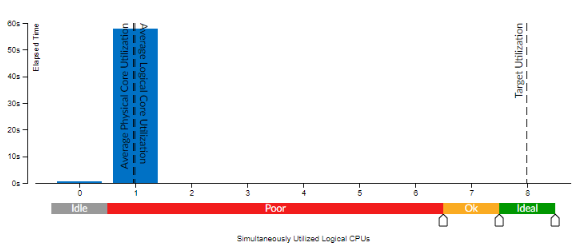
\includegraphics[width=13cm]{sekwencyjny_bezsita_2_MAX}
                    \caption{\gls{SPPLL} dla liczb z zakresu $2 .. MAX$}
                \end{figure}
                \begin{figure}[H]
                    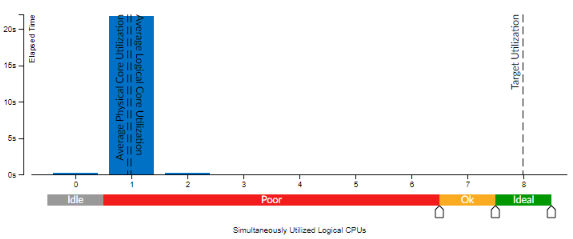
\includegraphics[width=13cm]{sekwencyjny_bezsita_2_MAX2}
                    \caption{\gls{SPPLL} dla liczb z zakresu $2 .. MAX / 2$}
                \end{figure}
                \begin{figure}[H]
                    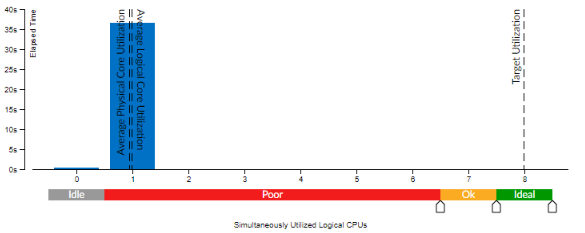
\includegraphics[width=13cm]{sekwencyjny_bezsita_MAX2_MAX}
                    \caption{\gls{SPPLL} dla liczb z zakresu $MAX / 2 .. MAX$}
                \end{figure}
            
            \subsubsection{Sekwencyjne Sito Erastotenesa - \gls{SSE}}
                \begin{figure}[H]
                    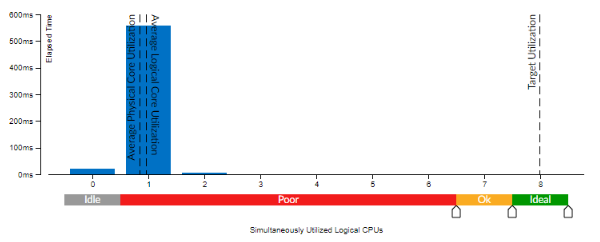
\includegraphics[width=13cm]{sekwencyjny_sito_2_MAX}
                    \caption{\gls{SSE} dla liczb z zakresu $2 .. MAX$}
                \end{figure}
                \begin{figure}[H]
                    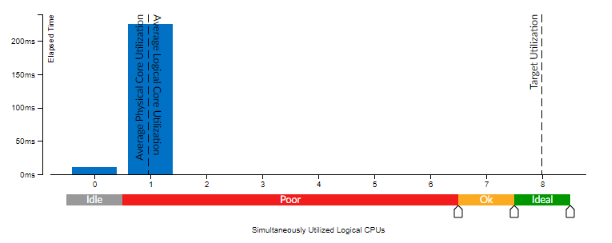
\includegraphics[width=13cm]{sekwencyjny_sito_2_MAX2}
                    \caption{\gls{SSE} dla liczb z zakresu $2 .. MAX / 2$}
                \end{figure}
                \begin{figure}[H]
                    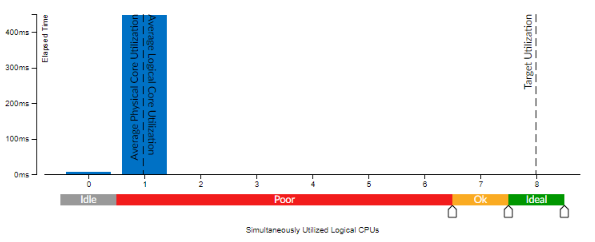
\includegraphics[width=13cm]{sekwencyjny_sito_MAX2_MAX}
                    \caption{\gls{SSE} dla liczb z zakresu $MAX / 2 .. MAX$}
                \end{figure}
        
            \subsubsection{Równoległe Naiwne Sito Erastotenesa wersja Funkcyjna}
                \begin{figure}[H]
                    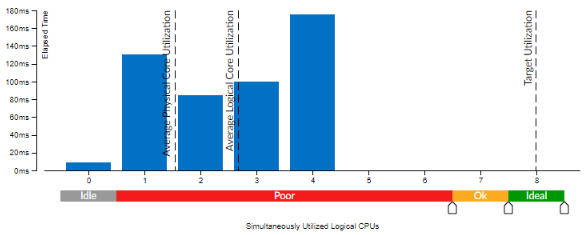
\includegraphics[width=13cm]{rownolegly_funcion4_2_MAX}
                    \caption{\gls{RNSEF} dla liczb z zakresu $2 .. MAX$ dla 4 procesorów logicznych}
                \end{figure}
                \begin{figure}[H]
                    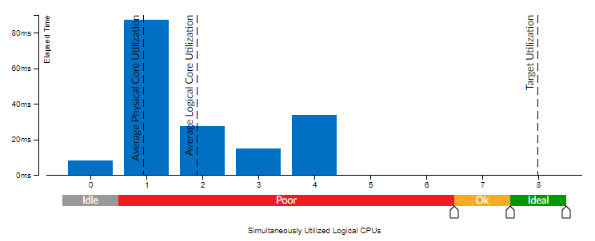
\includegraphics[width=13cm]{rownolegly_funcion4_2_MAX2}
                    \caption{\gls{RNSEF} dla liczb z zakresu $2 .. MAX / 2$ dla 4 procesorów logicznych}
                \end{figure}
                \begin{figure}[H]
                    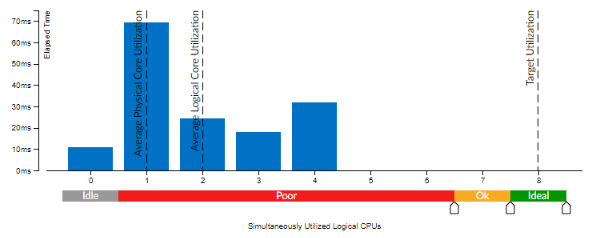
\includegraphics[width=13cm]{rownolegly_funcion4_MAX2_MAX}
                    \caption{\gls{RNSEF} dla liczb z zakresu $MAX / 2 .. MAX$ dla 4 procesorów logicznych}
                \end{figure}
                \begin{figure}[H]
                    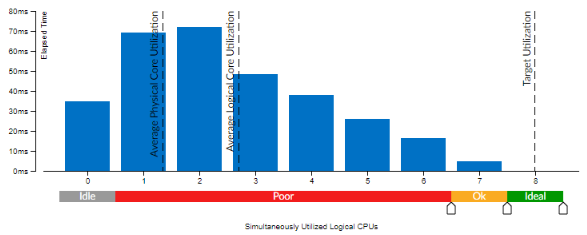
\includegraphics[width=13cm]{rownolegly_funcion8_2_MAX}
                    \caption{\gls{RNSEF} dla liczb z zakresu $2 .. MAX$ dla 8 procesorów logicznych}
                \end{figure}
                \begin{figure}[H]
                    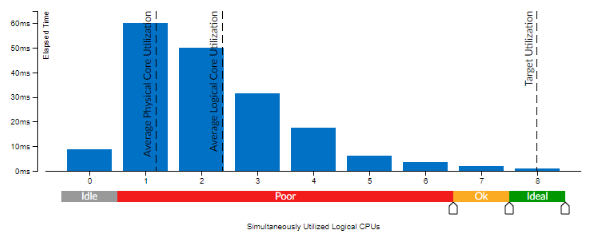
\includegraphics[width=13cm]{rownolegly_funcion8_2_MAX2}
                    \caption{\gls{RNSEF} dla liczb z zakresu $2 .. MAX / 2$ dla 8 procesorów logicznych}
                \end{figure}
                \begin{figure}[H]
                    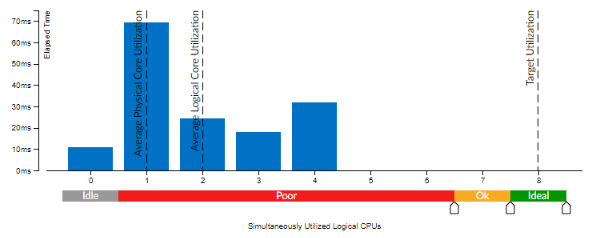
\includegraphics[width=13cm]{rownolegly_funcion8_MAX2_MAX}
                    \caption{\gls{RNSEF} dla liczb z zakresu $MAX / 2 .. MAX$ dla 8 procesorów logicznych}
                \end{figure}
                
            \subsubsection{Równoległe Optymalne Sito Erastotenesa wersja Funkcyjna}
                \begin{figure}[H]
                    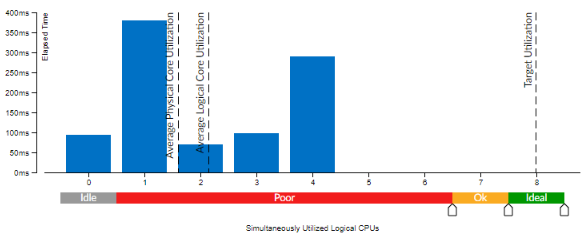
\includegraphics[width=13cm]{rownolegly_funcion_opt4_2_MAX}
                    \caption{\gls{ROSEF} dla liczb z zakresu $2 .. MAX$ dla 4 procesorów logicznych}
                \end{figure}
                \begin{figure}[H]
                    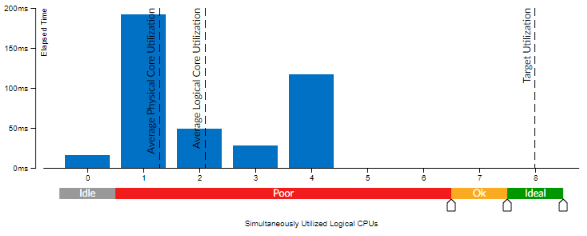
\includegraphics[width=13cm]{rownolegly_funcion_opt4_2_MAX2}
                    \caption{\gls{ROSEF} dla liczb z zakresu $2 .. MAX / 2$ dla 4 procesorów logicznych}
                \end{figure}
                \begin{figure}[H]
                    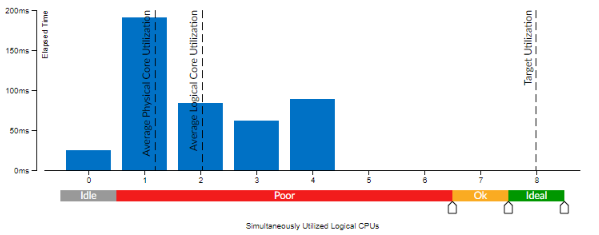
\includegraphics[width=13cm]{rownolegly_funcion_opt4_MAX2_MAX}
                    \caption{\gls{ROSEF} dla liczb z zakresu $MAX / 2 .. MAX$ dla 4 procesorów logicznych}
                \end{figure}
                \begin{figure}[H]
                    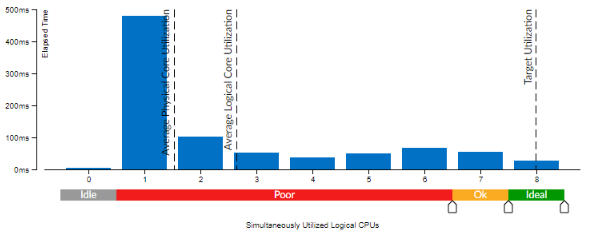
\includegraphics[width=13cm]{rownolegly_funcion_opt8_2_MAX}
                    \caption{\gls{ROSEF} dla liczb z zakresu $2 .. MAX$ dla 8 procesorów logicznych}
                \end{figure}
                \begin{figure}[H]
                    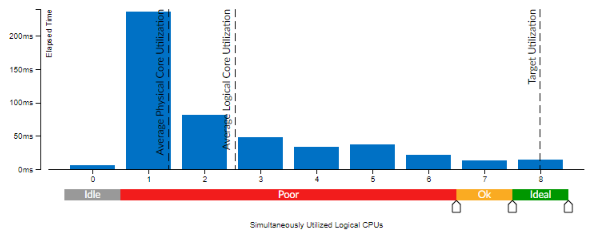
\includegraphics[width=13cm]{rownolegly_funcion_opt8_2_MAX2}
                    \caption{\gls{ROSEF} dla liczb z zakresu $2 .. MAX / 2$ dla 8 procesorów logicznych}
                \end{figure}
                \begin{figure}[H]
                    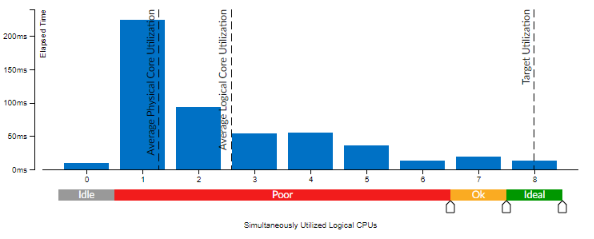
\includegraphics[width=13cm]{rownolegly_funcion_opt8_MAX2_MAX}
                    \caption{\gls{ROSEF} dla liczb z zakresu $MAX / 2 .. MAX$ dla 8 procesorów logicznych}
                \end{figure}
                
            \subsubsection{Równoległe Optymalne Sito Erastotenesa wersja Domenowa}
                \begin{figure}[H]
                    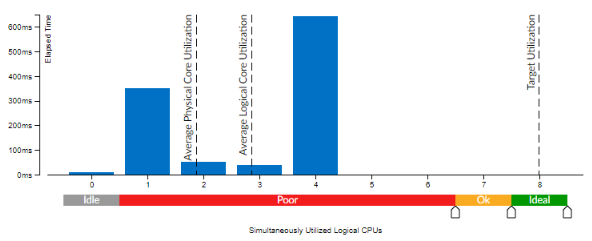
\includegraphics[width=13cm]{rownolegly_domain_opt4_2_MAX}
                    \caption{\gls{ROSED} dla liczb z zakresu $2 .. MAX$ dla 4 procesorów logicznych}
                \end{figure}
                \begin{figure}[H]
                    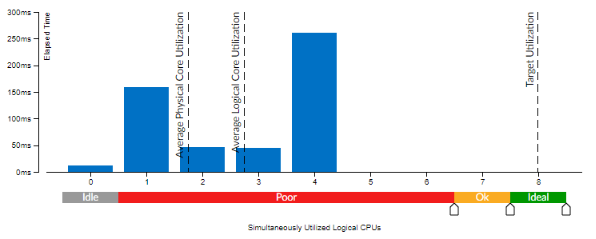
\includegraphics[width=13cm]{rownolegly_domain_opt4_2_MAX2}
                    \caption{\gls{ROSED} dla liczb z zakresu $2 .. MAX / 2$ dla 4 procesorów logicznych}
                \end{figure}
                \begin{figure}[H]
                    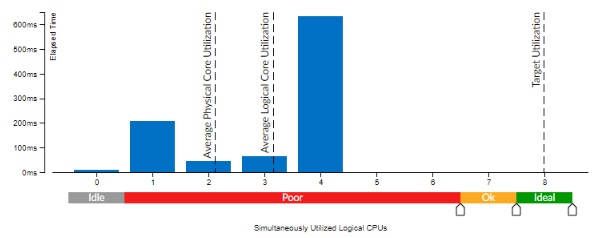
\includegraphics[width=13cm]{rownolegly_domain_opt4_MAX2_MAX}
                    \caption{\gls{ROSED} dla liczb z zakresu $MAX / 2 .. MAX$ dla 4 procesorów logicznych}
                \end{figure}
                \begin{figure}[H]
                    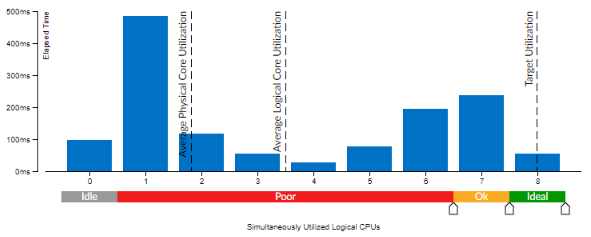
\includegraphics[width=13cm]{rownolegly_domain_opt8_2_MAX}
                    \caption{\gls{ROSED} dla liczb z zakresu $2 .. MAX$ dla 8 procesorów logicznych}
                \end{figure}
                \begin{figure}[H]
                    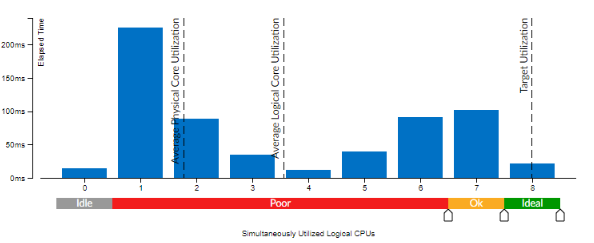
\includegraphics[width=13cm]{rownolegly_domain_opt8_2_MAX2}
                    \caption{\gls{ROSED} dla liczb z zakresu $2 .. MAX / 2$ dla 8 procesorów logicznych}
                \end{figure}
                \begin{figure}[H]
                    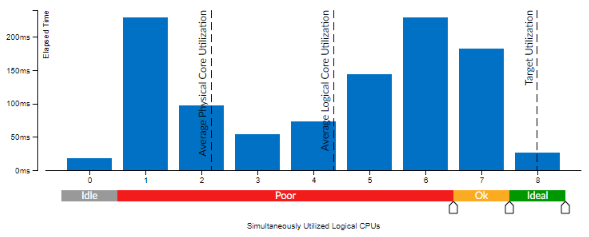
\includegraphics[width=13cm]{rownolegly_domain_opt8_MAX2_MAX}
                    \caption{\gls{ROSED} dla liczb z zakresu $MAX / 2 .. MAX$ dla 8 procesorów logicznych}
                \end{figure}
                
            \subsubsection{Równoległe Naiwne Pełne Przeglądanie Listy Liczb}
                \begin{figure}[H]
                    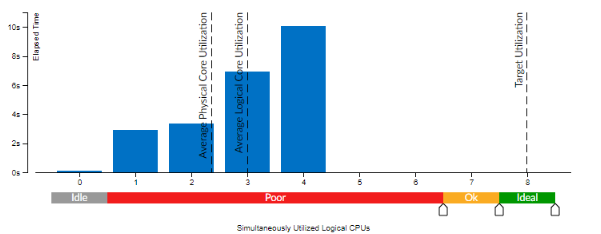
\includegraphics[width=13cm]{rownolegly_domain_bezsita4_2_MAX}
                    \caption{\gls{RNPPLL} dla liczb z zakresu $2 .. MAX$ dla 4 procesorów logicznych}
                \end{figure}
                \begin{figure}[H]
                    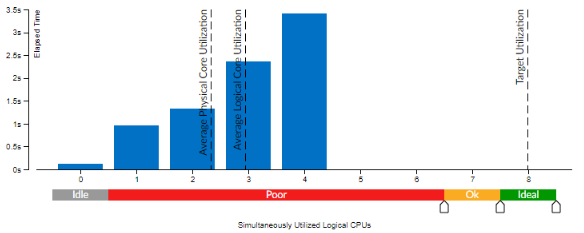
\includegraphics[width=13cm]{rownolegly_domain_bezsita4_2_MAX2}
                    \caption{\gls{RNPPLL} dla liczb z zakresu $2 .. MAX / 2$ dla 4 procesorów logicznych}
                \end{figure}
                \begin{figure}[H]
                    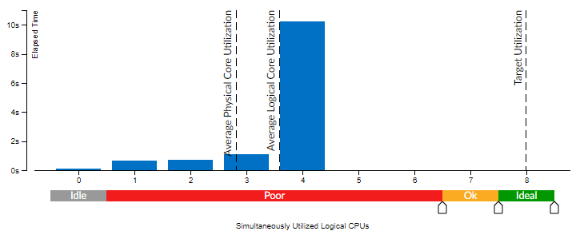
\includegraphics[width=13cm]{rownolegly_domain_bezsita4_MAX2_MAX}
                    \caption{\gls{RNPPLL} dla liczb z zakresu $MAX / 2 .. MAX$ dla 4 procesorów logicznych}
                \end{figure}
                \begin{figure}[H]
                    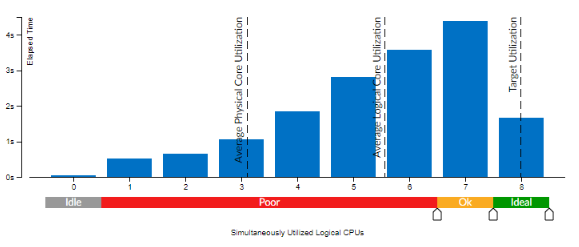
\includegraphics[width=13cm]{rownolegly_domain_bezsita8_2_MAX}
                    \caption{\gls{RNPPLL} dla liczb z zakresu $2 .. MAX$ dla 8 procesorów logicznych}
                \end{figure}
                \begin{figure}[H]
                    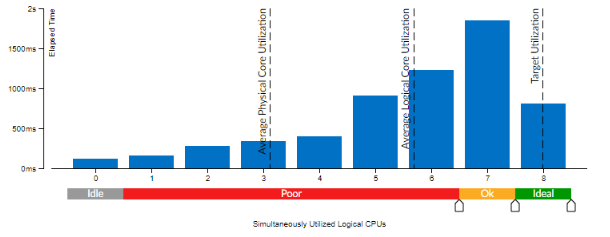
\includegraphics[width=13cm]{rownolegly_domain_bezsita8_2_MAX2}
                    \caption{\gls{RNPPLL} dla liczb z zakresu $2 .. MAX / 2$ dla 8 procesorów logicznych}
                \end{figure}
                \begin{figure}[H]
                    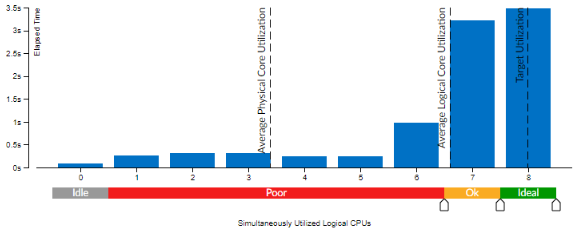
\includegraphics[width=13cm]{rownolegly_domain_bezsita8_MAX2_MAX}
                    \caption{\gls{RNPPLL} dla liczb z zakresu $MAX / 2 .. MAX$ dla 8 procesorów logicznych}
                \end{figure}
                
            \subsubsection{Równoległe Optymalne Pełne Przeglądanie Listy Liczb}
                \begin{figure}[H]
                    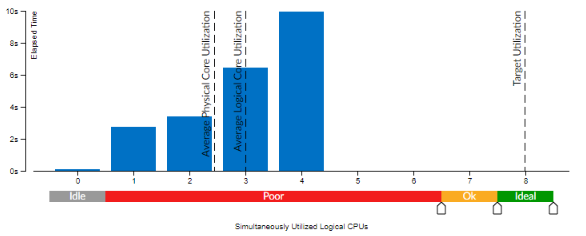
\includegraphics[width=13cm]{rownolegly_funcion_bezsita4_2_MAX}
                    \caption{\gls{ROPPLL} dla liczb z zakresu $2 .. MAX$ dla 4 procesorów logicznych}
                \end{figure}
                \begin{figure}[H]
                    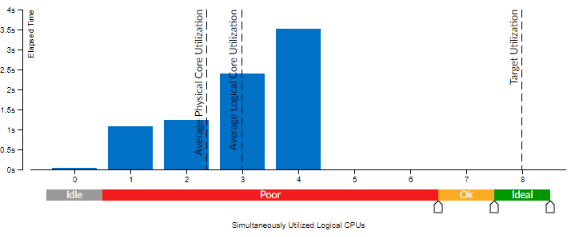
\includegraphics[width=13cm]{rownolegly_funcion_bezsita4_2_MAX2}
                    \caption{\gls{ROPPLL} dla liczb z zakresu $2 .. MAX / 2$ dla 4 procesorów logicznych}
                \end{figure}
                \begin{figure}[H]
                    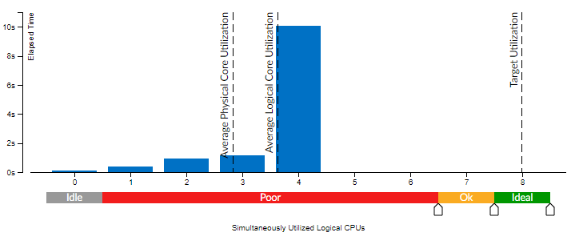
\includegraphics[width=13cm]{rownolegly_funcion_bezsita4_MAX2_MAX}
                    \caption{\gls{ROPPLL} dla liczb z zakresu $MAX / 2 .. MAX$ dla 4 procesorów logicznych}
                \end{figure}
                \begin{figure}[H]
                    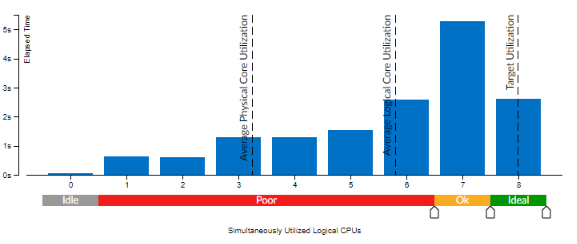
\includegraphics[width=13cm]{rownolegly_funcion_bezsita8_2_MAX}
                    \caption{\gls{ROPPLL} dla liczb z zakresu $2 .. MAX$ dla 8 procesorów logicznych}
                \end{figure}
                \begin{figure}[H]
                    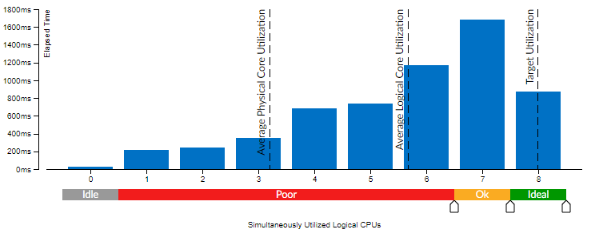
\includegraphics[width=13cm]{rownolegly_funcion_bezsita8_2_MAX2}
                    \caption{\gls{ROPPLL} dla liczb z zakresu $2 .. MAX / 2$ dla 8 procesorów logicznych}
                \end{figure}
                \begin{figure}[H]
                    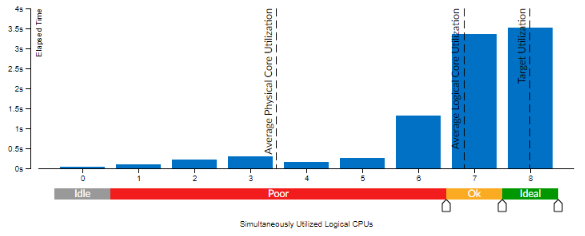
\includegraphics[width=13cm]{rownolegly_funcion_bezsita8_MAX2_MAX}
                    \caption{\gls{ROPPLL} dla liczb z zakresu $MAX / 2 .. MAX$ dla 8 procesorów logicznych}
                \end{figure}
        
    
    \clearpage
    \printnoidxglossaries
\end{document}